\chapter{Integration of resting-state networks during reading}

\section{Motivation}

% Reorganization may also index reading skill
In Study 1, we began building an argument that the brain compartmentalizes its cognitive functions because this improves cognitive efficiency, both for specific tasks and for integrating across the whole-brain network. We found this to be true in the case of reading fluency: global modularity is positively related to reading skill, even when controlling for verbal intelligence and motion. However, the brain network is not static but rather  changes in response to the demands made upon it. Therefore, evaluating the brain \textit{while} it is reading is critical for understanding how its organization supports fluency. 

% Task-evoked network architecture
While resting-state functional connectivity is thought to provide insights into a relatively stable intrinsic architecture, \textit{task-evoked} functional connectivity measures network organization in response to an environmental demand. The degree of reconfiguration is physiologically limited: the BOLD signal change during a task is only about 1 percent \citep{Fox2007}, and there are underlying structural constraints such as white matter connectivity \citep{Sui2014}. Nevertheless, there is a large degree of flexibility to reconfigure the functional network based on the demands of the task. One study, for example, compared a finger-tapping to working memory task. Using measures of modularity and participation coefficient, they found that within-network communication was critical for the motor task, whereas between-network communication was important for working memory \citep{Cohen2016}. This supports a hypothesis that tasks can operate on multiple levels: high connectivity within-module for sensorimotor tasks, and distributed for ones that require higher-order skills. The ability to flexibly switch between high- and low-modularity states may thus be an important trait.

% Effects on network organization during reading
Reading, and especially reading comprehension, spans both levels of cognitive activity. On the one hand, readers continuously receive visual stimuli and transform them into auditory and semantic representations. These representations must then be kept in memory, evaluated for relevance and updated when necessary \citep{Maguire1999}. In general, task-evoked network architecture induces a decrease in modularity \citep{Cole2014}, and this decrease is associated with active engagement and awareness of the task at hand \citep{Godwin2015}. Other studies have shown that the extent of the modularity is related to the novelty and expertise at the task \citep{Bassett2015}. This has not, however, been related to individual differences in those broader cognitive skills.

% Relationship of reading skill to modularity change
A complementary question is whether the relationship between reading skill and network modularity \textit{while reading} should remain the same. One hypothesis is that, if cross-network communication is critical to reading, better readers should exhibit a much less modular organization while reading than poor readers. However, there is evidence from univariate analyses of brain activation that would suggest the opposite: compared to poor readers, expert readers show \textit{less} activation in many reading-related areas during reading tasks \citep{Christodoulou2014}. In the context of interactive specialization, this is explained by the increased efficiency of information transfer within an established network. If the resting-state network architecture represents an efficient baseline, then expert readers may be expected to deviate from it less.

% How does activity relate to reading? 
It has been well-established that during reading, brain activity patterns span a wide range of networks and both hemispheres, especially as texts become longer and more complex \citep{Rimrodt2009, Xu2005}. However, less understood is the relationship between task-activity and changes to an area's role in the network. Although hub regions of the brain are known to be important for cognitive functioning, implicated in a wide variety of processes and localize predominantly onto association cortices, we are not aware of any studies that have directly compared their hub role to their BOLD response in a specific task. That is, does the ``activation'' of a hub node correspond to its connecting of more areas, or does it reflect a specific in the traditional sense corresponds to increased engagement with many areas, or if it reflects primarily local processing. The answer may be region- and task-dependent: visual areas may performing local processing, whereas activation of FPN areas may indicate the linking of two networks. 

% This study's objectives
Reading comprehension is thus an excellent model task for understanding how task-evoked changes to network architecture vary throughout the brain and along reading skill. First, we validate our task with a traditional univariate analysis. Next, we describe the global changes to different aspects of network architecture during each condition. Then, we pinpoint which brain areas and RSNs that drive the changes to network architecture, and investigate the relationship between these changes and individual differences in reading skill. 


\section{Methods}

\subsection{Participants}

Participants were drawn from the same cohort of subjects included in Study 1, and identical inclusion criteria for both demographic and scan motion were applied. However, additional measures related to the performance of the task were levied as described below. A total of 47 unique subjects and 88 scan sessions were included in the analysis. Their demographics are described in Table \ref{table:ch3-participants}.

\begin{table}
	\renewcommand{\tabcolsep}{0.09cm}
	\centering
	\begin{tabular}{lc}
\toprule 
Measure & Subjects \\ 
\midrule 
No. Participants				& 42 \\ 
No. Scan Runs					& 164 \\ 
Gender  						& 25 F \\ 
Age at Scan 					& 10.5 (0.3)  \\ 
WASI Full-Scale IQ  			& 111.0 (16.2) \\ 
TOWRE - Total Word Efficiency 	& 104.6 (18.5) \\ 
\bottomrule 
\end{tabular}
	\caption[Participant demographics for Study 2]{Participant demographics for Study 2. Subjects include all of those from Study 1, and three additional ones who had sufficiently high quality task-fMRI scans.}
	\label{table:ch3-participants}
\end{table}


\subsection{MRI acquisition and task design}

Participants performed up to four runs of a language comprehension task, which was crossed on two conditions: the modality of presentation (listening or reading) and the passage genre (expository or narrative). Functional MRI acquisition parameters were identical to Study 1 with the exception of scan duration, which was increased to a total of 250 dynamic volumes for each run. 

For the present analysis, only the ``reading'' scans were considered, and the effects of genre on brain activation were ignored, as they are balanced out within the majority of subjects. (6 subjects had only a single genre used for analysis.) In the following paragraphs, however, we will describe the experiment design in its entirety, as it will be relevant to subsequent analyses.

Each fMRI run had two baseline conditions: a modality-specific baseline task and a resting-state block with a fixation cross. At the conclusion of the comprehension portion of each experiment, two images were presented, and subjects were asked to decide if the image was related to the passage. (e.g., Is a picture of a cake with candles related to a story about a birthday party?) The order and duration for each block varied slightly across runs but was approximately: paragraph 1 (60 s), baseline 1 (60 s), paragraph 2 (60 s), baseline 2 (60 s), and resting-state (270 s). Total scan time was 550 s for each run. See Fig. \ref{fig:ch3-task-design} for a schematic describing the visual task.

\begin{figure}[t]
	\centering
	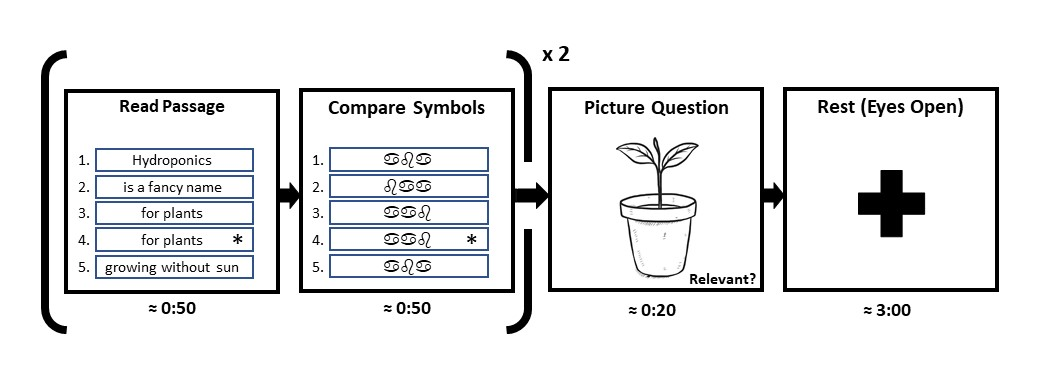
\includegraphics[width=6in]{ch3-task-design}
	\caption[Schematic of the reading comprehension task]{Schematic of the reading comprehension task. Subjects were presented two blocks of passage reading and a symbol comparison tasks, which were followed by a brief comprehension question and a resting block. Starred stimuli in the reading and symbols conditions represent ``repeat'' stimuli, and a participant is asked to click a button when they detect one. The total duration of each scan run was 550 seconds.}
	\label{fig:ch3-task-design}
\end{figure}

To create a more naturalistic reading experience than single word presentation \citep{Rayner1998}, passages were presented in syntactic phrases ranging from 1-7 words in length. The interval between each stimulus was jittered to allow for event-related analyses (range: 275 – 4000 ms), although these effects were not examined here.

The sensory baseline condition was altered according to modality. For the reading runs, three non-alphanumeric symbols were displayed horizontally (two types), and their presentation time was matched to the passage phrases. Spacing between symbols was randomly alternated to replicate the variable phrase lengths in the passage condition. For the listening runs, three tones (two frequencies) were played in sequence, with a new set of tones beginning at the same intervals as the corresponding passage presentation. 

To monitor attention, 4 to 8 percent of the stimuli within each passage or symbols block were randomly repeated on two consecutive screens.  Participants pressed a button with their right thumb when they detected a repeated phrase, symbol or tone configuration. Additionally, at the conclusion of each passage, a picture was presented on the screen, and subjects were asked to identify whether the picture had any relationship to the passage (e.g., a picture of a mushroom for a passage about fungi). 

To assess performance, we analyzed three measures: in-scanner attention, in-scanner comprehension, and post-scan recall. To assess attention for the ``repeated stimulus'' task, we used the $D`$ summary measure. It is calculated as:

$$
D^\prime = Z_{true\ positive} - Z_{false\ positive}
$$

Individual scan runs with a $D`$ value less than 2 were excluded from analysis. The in-scanner comprehension measure was the number (either 0, 1, or 2) of questions correctly answered. To assess recall after the scan, each child was asked to recite as much of the passage as they could remember, and their answers were mapped to actual phrases present in the chapter. 

In total, there were 4 passages (2 listening and 2 reading), each leveled to a third grade difficulty level and balanced on word measures such as concreteness and cohesiveness.  All subjects were trained on the task in a mock scanner prior to the actual scan. 


\subsection{Activation analyses}

Whole-brain fMRI analyses were performed using tools from the FMRIB Software Library (version 5.0.9). For each session, the following pre-processing steps were performed:  slice-time correction, motion correction to the initial fMRI volume, high-pass filtering at 0.08 Hz, boundary-based registration to the subject's structural image, and normalization to 2 mm MNI 152 standard space. To mitigate the effects of motion on our analyses, we regressed out 6 continuous motion parameters and scrubbed out outlier volumes. We defined an outlier volume as any in which the root-mean-square framewise displacement exceeded 0.7 mm. We removed scan runs where more than 20 percent of the fMRI volumes were considered outliers.

All task conditions were convolved with the double-gamma hemodynamic response function to generate design matrices for each fMRI run. Two first-level contrasts were of interest: the main effect of passage comprehension (``reading vs. rest''), and the contrast of passage comprehension vs. the sensory baseline (``reading vs. symbols''). Repeated stimuli and the picture comprehension task were modelled out.

Reading effects were estimated at the subject-level using fixed effects analysis. These were carried over into group-level analyses using non-parametric methods implemented in FSL’s \textit{randomise} tool with threshold-free cluster enhancement. For each group-level analysis, we performed 5000 permutations and report results with \textit{p} \textless 0.05. 

To understand our univariate results as a function of system-level activation, we also extracted activation values from each of the 264 connectome nodes, and summarized the activity of each intrinsic RSN.

\subsection{Network analyses}

For graph theory analyses, network estimation was performed in the \textit{Conn: Functional Connectivity Toolbox} (version 17f) \citep{WhitfieldGabrieli2012}. As in Study 1, for each scan run, the BOLD activity at each node was denoised using the anatomical CompCorr method, which regresses out background noise from white matter and cerebrospinal fluid tissue. We also regressed out 12 continuous measures of motion were also included, all outlier timepoints, and the effect of all task conditions (i.e., reading, symbols, and rest). The timeseries was then high-pass filtered at 0.01 Hz.

Whole-brain connectomes for each condition were created by estimating the functional connectivity between each node using a weighted general linear model. For connection-level analyses, these values were compared directly across subjects and conditions. For graph theory analyses, the array of all node connections was thresholded to keep the top 5 percent of connections, resulting in a much sparser representation. This threshold was also tested at ranges from 2 percent to 10 percent. These arrays were then characterized using the previously described graph theory measures: modularity, participation coefficient, and path length.

To investigate the rewiring of the network at the RSN-level, we compared the number of connections across each RSN relationship at each condition. For each pair of networks, we computed a paired $t$-test between the total number of connections between the networks to determine whether there were more in one or the other condition. This resulted in a 13 by 13 RSN-level connectivity array. Connectivity changes were performed at eaech of the 9 thresholds, and relationships that showed significant changes ($p < 0.05$, uncorrected) in at least 7 of the 9 thresholds were included in the rewiring diagram.


\section{Results}

\subsection{Behavioral results}

47 subjects (88 scan runs) met the attention and motion criteria for inclusion in the analysis. (5 subjects and 15 scan runs were excluded.) The distribution of performance and motion criteria are illustrated in Figure \ref{fig:ch3-task-performance}. 

\begin{figure}[t]
	\centering
	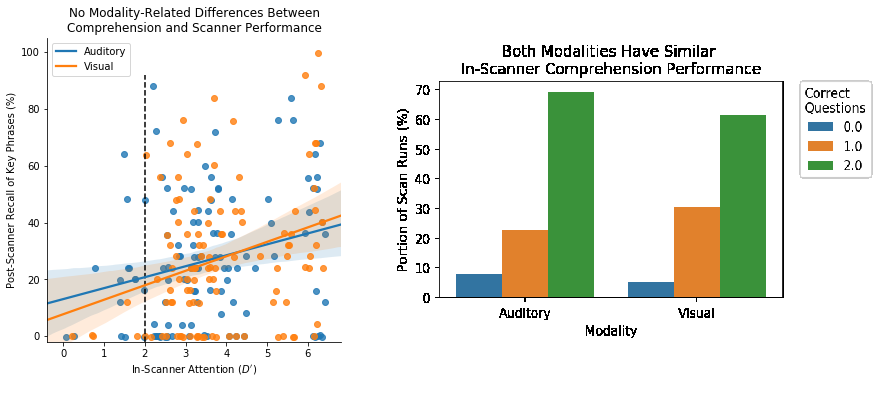
\includegraphics[height=3in]{ch3-task-performance}
    \caption[Description of scan motion quality and task performance]{Scatterplot summarizing the relationship between scan motion quality and task performance. The $D^\prime$ score measures performance based on both active (correctly identifies repeats) and passive (few false alarm clicks) metrics. The frame-wise displacement measure also accounts for outlier volumes which are regressed out during analysis.}
	\label{fig:ch3-task-performance}
\end{figure}

\subsection{Activation results}

Figure \ref{fig:ch3-reading-brain-activations} demonstrates the range of language-related areas were activated during reading comprehension. Compared to the symbols baseline, reading-related activation spanned the inferior frontal gyrus, angular gyrus, premotor cortex, middle temporal gyrus and the superior frontal gyrus. Activation patterns were robustly present on both hemispheres but extended further and with greater intensity on the left hemisphere. There were also a number of areas that were more active in the sensory and resting state, particularly in the dorsal attention network and anterior dorsolateral prefrontal cortex.

\begin{figure}[t]
	\centering
	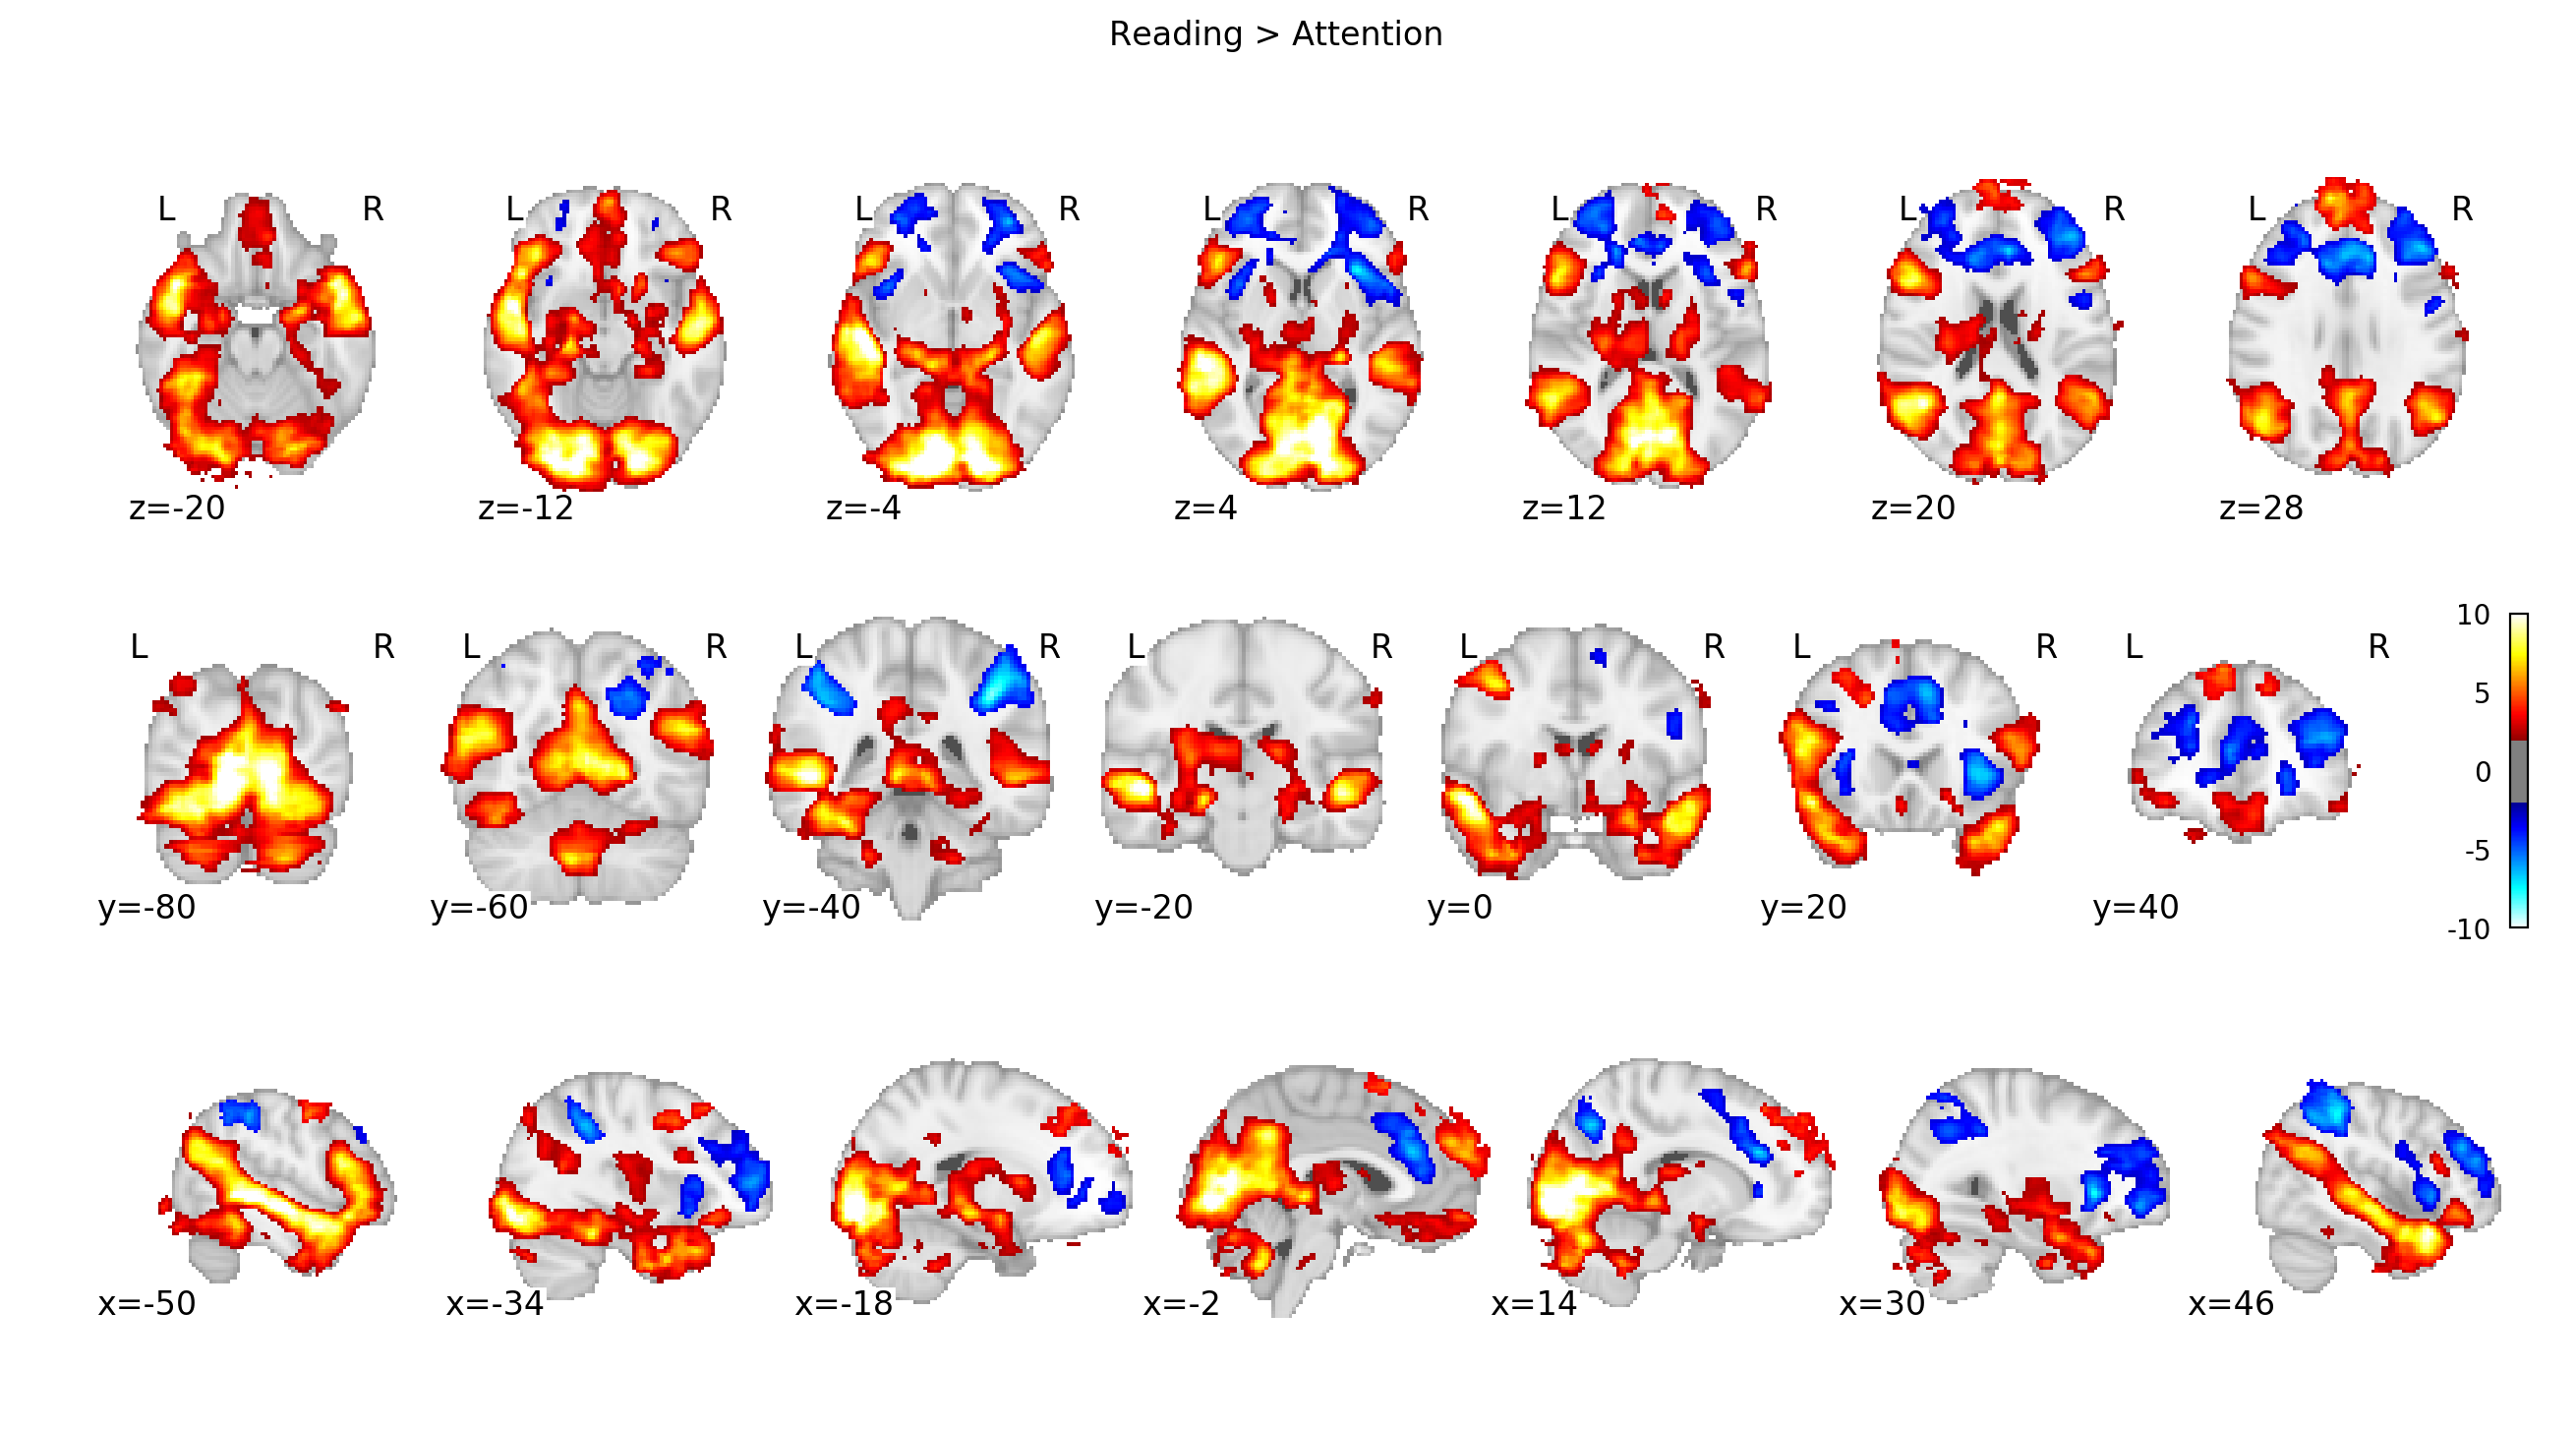
\includegraphics[width=6in]{ch3-reading-brain-activations}
    \caption[A range of language-related areas were activated during reading comprehension]{A range of language-related areas were activated during reading compreh ension. The above figures show axial, coronal and sagittal views of the ``reading vs. symbols'' activation contrast. Reading-related activations span expected areas, including left fusiform, middle temporal and inferior frontal gyri, but also extend into right hemisphere homologues and the cerebellum. Results are thresholded at $p < 0.05$ using threshold-free cluster enhancement (5000 permutations).}
	\label{fig:ch3-reading-brain-activations}
\end{figure}

To understand RSN-level trends in activation, we also examined the results when projected onto the 264 nodes in the connectome parcellation. Compared to the resting baseline, the ventral attention, visual and default mode networks had the greatest number of ``active'' nodes. It is also notable that the ``uncertain'' nodes were highly engaged. These nodes had variable activity that made them impossible to classify consistently in the original paper \citep{Power2011}. Their engagement may reflect the important role of functionally diverse regions in the execution of reading comprehension. On the other end, the memory retrieval, salience and cingulo-opercular networks exhibited decreased activity compared to rest. See Figure \ref{fig:ch3-reading-connectome-activations} for a diagram of these activations by RSN. 

\begin{figure}[t]
	\centering
	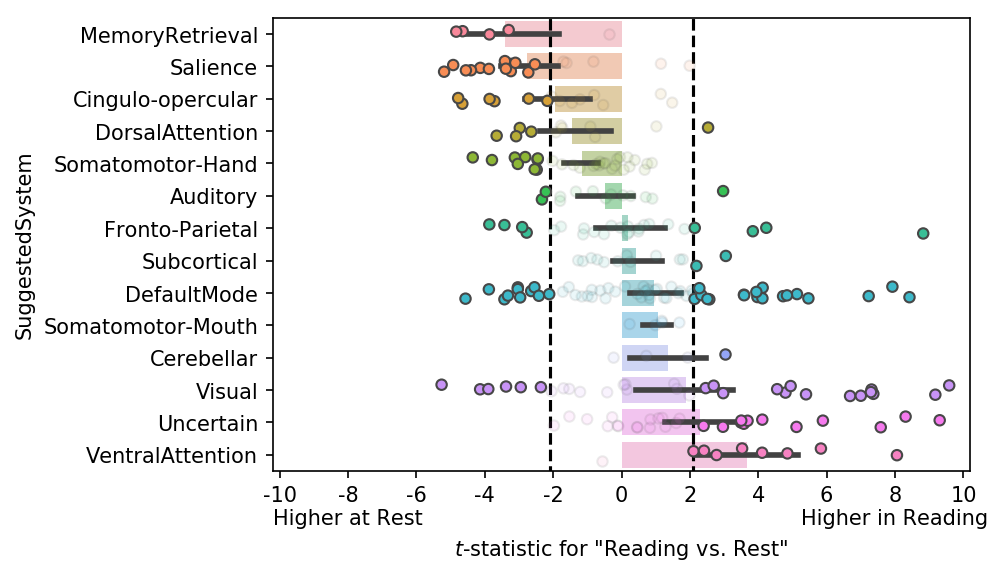
\includegraphics[height=3in]{ch3-reading-connectome-activations}
    \caption[Distribution of reading-related activity among RSN nodes]{Distribution of reading-related activity among connectome nodes, grouped by RSN. Each point represents a single node, while bars represent the aggregate mean for each RSN. Visual and ventral attention networks showed the most network-level activity in reading, although large portions of the default mode and fronto-parietal network were also robustly related. Cingulo-opercular, memory retrieval and salience networks showed decreases. Dashed lines represent $p < 0.05$, uncorrected.}
	\label{fig:ch3-reading-connectome-activations}
\end{figure}


\subsection{Network results}

Next, we examined changes to global network architecture. Figure \ref{fig:ch3-comprehension-graph-theory-all} summarizes the subject-level changes (as well as significance values) in modularity, participation coefficient, and path length. Overall, the effect was one of increased integration across RSNs during reading comprehension. Relative to rest, both reading comprehension reduced the global modularity and increased the participation coefficient. The magnitude of the effect in reading comprehension was also greater than that of the sensory condition. The path length within each RSN did not significantly change across condition, suggesting that the modular organization of the brain was not disrupted.  However, there were significant increases in the between-RSN path length corresponding to greater efficiency of transferring information between these disparate systems.

\begin{figure}[t!]
	\centering
	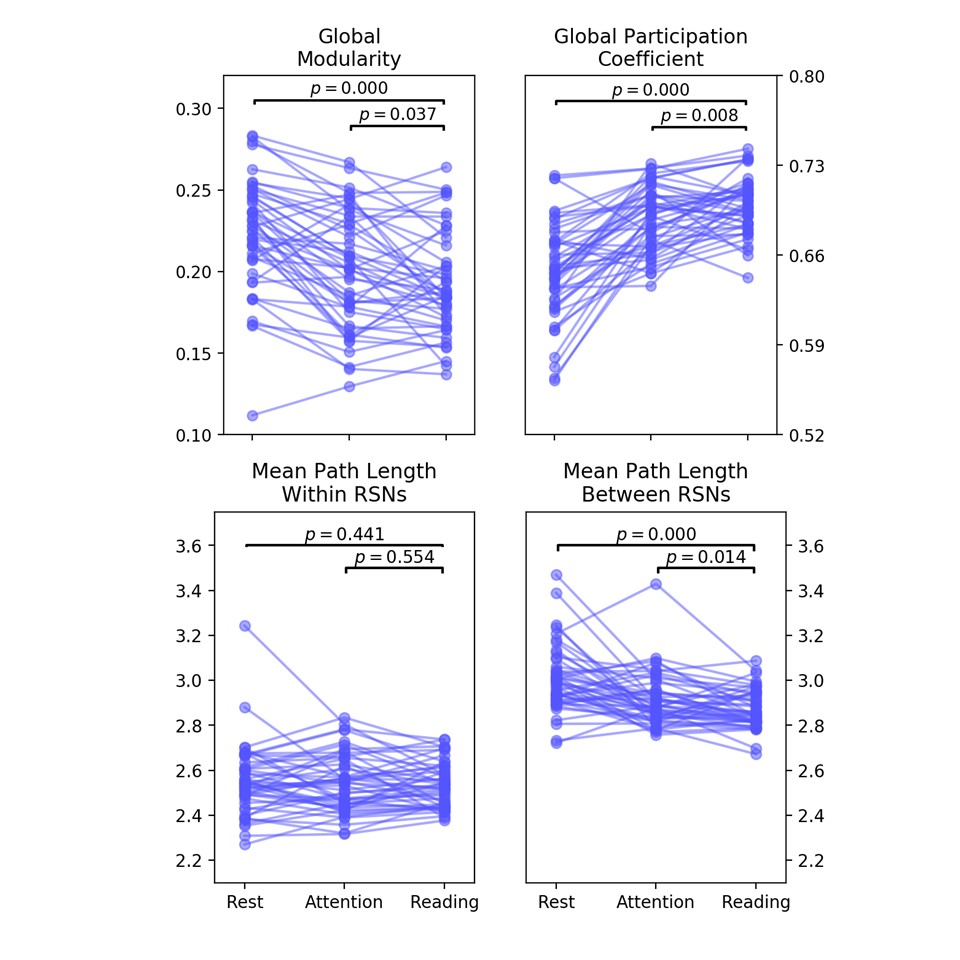
\includegraphics[width=5.3in]{ch3-comprehension-graph-theory-all}
    \caption[Reading induces a more integrated global network architecture]{Reading induces a more integrated global network architecture. Each set of connected points represents a single subject. Compared to rest and the baseline symbols task, reading comprehension increased global measures related to RSN integration. Notably, the only measure not significantly changed during task was the within-RSN path length.}
	\label{fig:ch3-comprehension-graph-theory-all}
\end{figure}

Network-level trends in task-evoked differences, presented in Figure \ref{fig:ch3-rsn-condition-effects}, were largely consistent with global effects. However, a few findings are worth noting: compared to rest, reading was marked by large decreases in modularity of the visual, dorsal attention and default mode networks. However, the increases to participation coefficient were global. Compared to the symbols task, network-level changes were modest, and the global differences were driven by reduced modularity in the default mode and fronto-parietal networks and increased participation of memory retrieval and default mode networks.

\begin{figure}[t!]
	\centering
	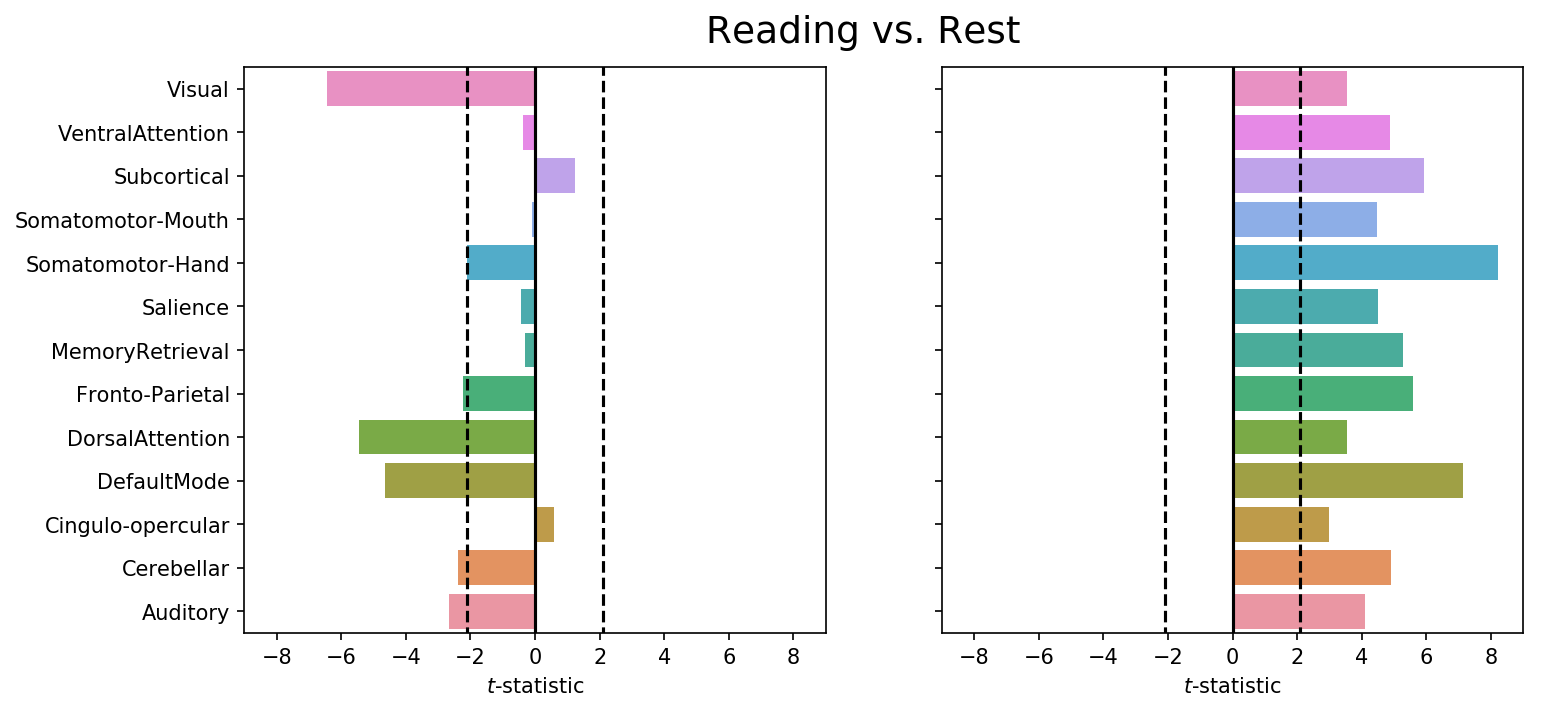
\includegraphics[width=6in]{ch3-rsn-condition-effects-rest}
	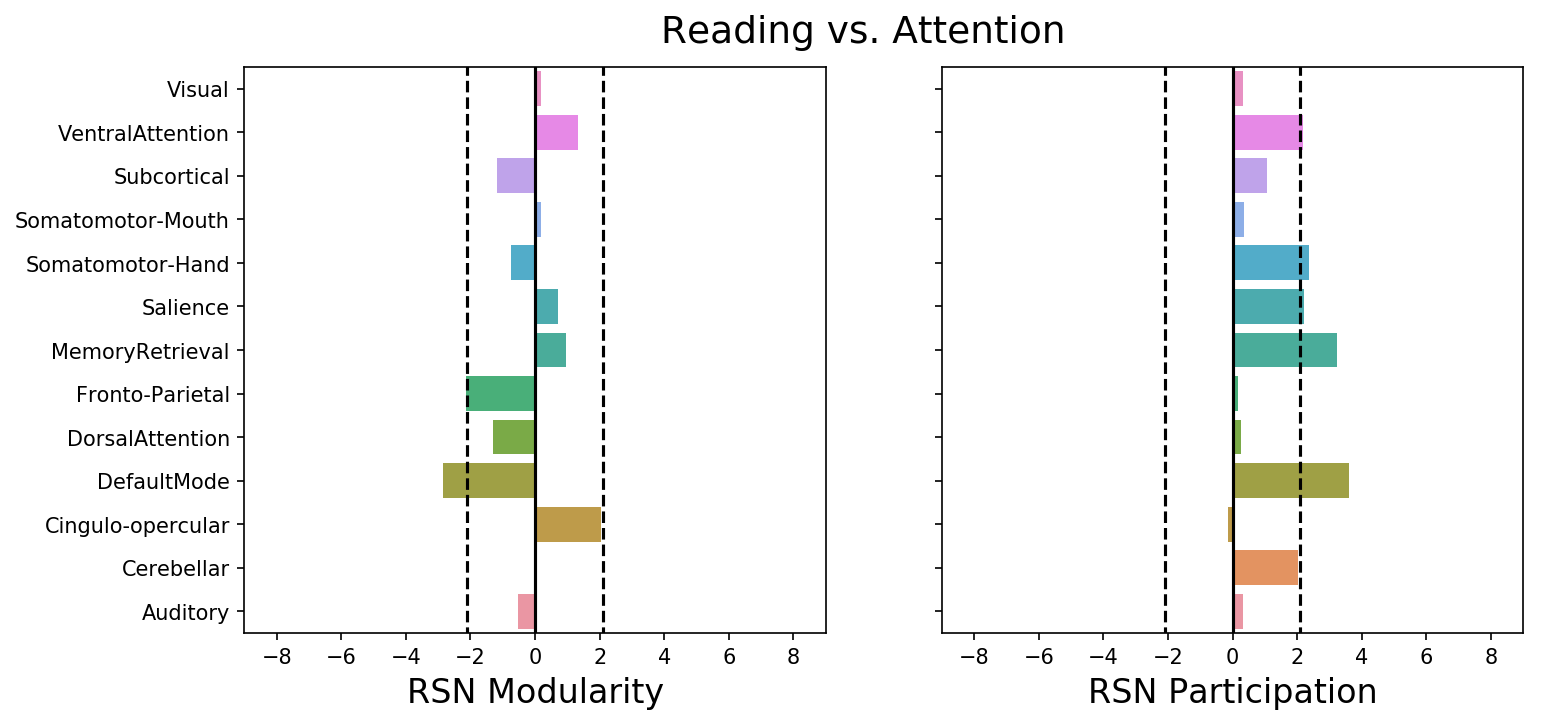
\includegraphics[width=6in]{ch3-rsn-condition-effects-attn}
    \caption[RSN-level trends in task-evoked networks]{RSN-level trends in task-evoked networks. Changes to modularity were driven by the de-clustering of the visual, dorsal attention and default mode networks. For the participation coefficient, network-level trends in task-evoked differences to graph theory measures were largely related to global trends. There were many fewer significant changes in the ``reading vs. symbols'' contrast. Dashed lines represent uncorrected significance thresholds of $p < 0.05$.}
	\label{fig:ch3-rsn-condition-effects}
\end{figure}

Specific relationships between RSNs are made apparent when comparing when examining the ``rewiring'' diagram comparing rest and reading (Figure \ref{fig:ch3-comprehension-reorganization}). During rest, there are many more within-module connections in the sensory systems, dorsal attention and default mode networks. When reading, however, between-network connections increase across many between-network relationships and none within-network relationships. There is a modest breakdown of the modularity during reading, in which there is a global increase in integration across RSNs.

\begin{figure}[t!]
	\centering
	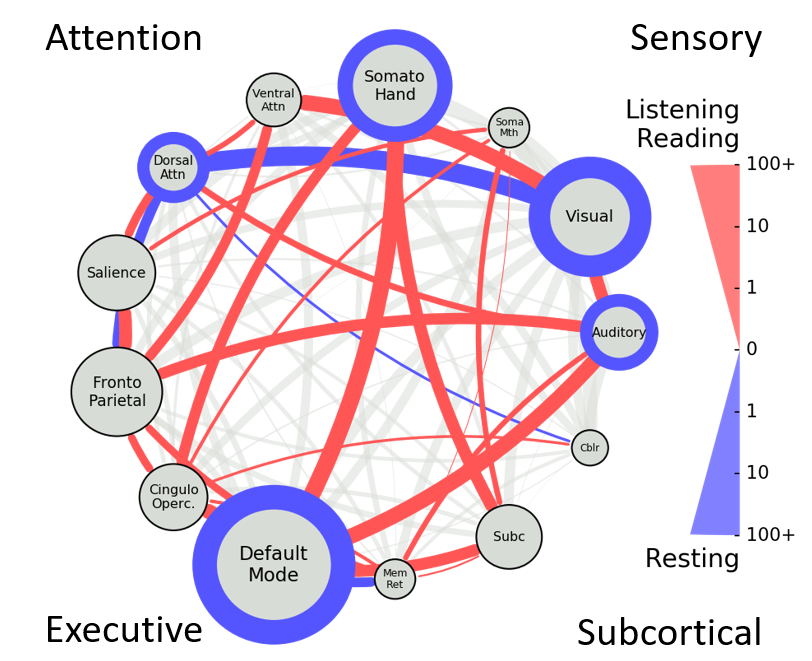
\includegraphics[height=4in]{ch3-comprehension-reorganization}
    \caption[Rewiring of RSNs during reading]{Rewiring diagram showing the changes in connectivity between networks during reading. During rest, there are many more within-module connections in the sensory systems, dorsal attention and default mode networks. During reading, however, between-network connections increase across many between-network relationships and none within-network relationships. That is, the brain becomes more integrated.}
	\label{fig:ch3-comprehension-reorganization}
\end{figure}

Decreases in modularity are coupled by increases in the participation of specific nodes. To address whether the areas that are activated during reading (in the traditional univariate sense) are also the areas driving integration, we correlated the two variables at the node level. Interestingly, we found that nodes that were more activated in reading tended to be those with lower participation coefficients ($r = -0.434$, $p < 0.001$). Nodes with high participation coefficients tended to be deactivated relative to rest, although a few of these hub-like areas were also activated. (This effect can be seen in Figure \ref{fig:ch3-node-participation-to-activation}). One noteworthy hub area was the left posterior middle temporal gyrus (MNI coordinates: $x=-56$, $y=-50$, $z=10$). It was the most hub-like area at rest ($PC > 0.7$) that was also activated during the task ($t$-stat = 8.1). 

% Color the nodes by "activated vs inactivated"
\begin{figure}[t]
	\centering
	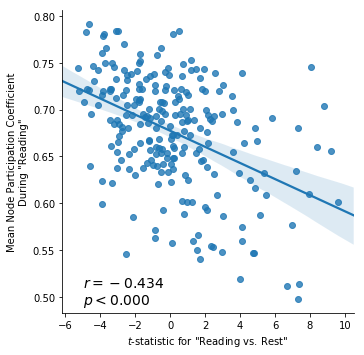
\includegraphics[width=4in]{ch3-node-participation-to-activation}
    \caption[Univariate activity is anti-correlated with participation coefficients]{Univariate activity is anti-correlated with participation coefficients. Nodes with high participation coefficients tended to be deactivated relative to rest, although a few of these hub-like areas were also activated.}
	\label{fig:ch3-node-participation-to-activation}
\end{figure}

Finally, we sought to replicate our previous finding relating resting-state modularity with reading, and to determine whether this relationship would change in the task-evoked network. For the reading and rest task conditions, we regressed the global modularity against the TOWRE Total Word Efficiency standard score. We replicated the results of Study 1 using the shorter rest condition from our task ($r_{rest} = 0.432$, $p < 0.01$), and we also found that the relationship held in the reading condition ($r_{read} = 0.494$, $p < 0.01$) (Figure \ref{fig:ch3-modularity-reading-by-condition}). There was no relationship between reading skill and the \textit{change} in modularity between reading and rest, however.  

\begin{figure}[t]
	\centering
	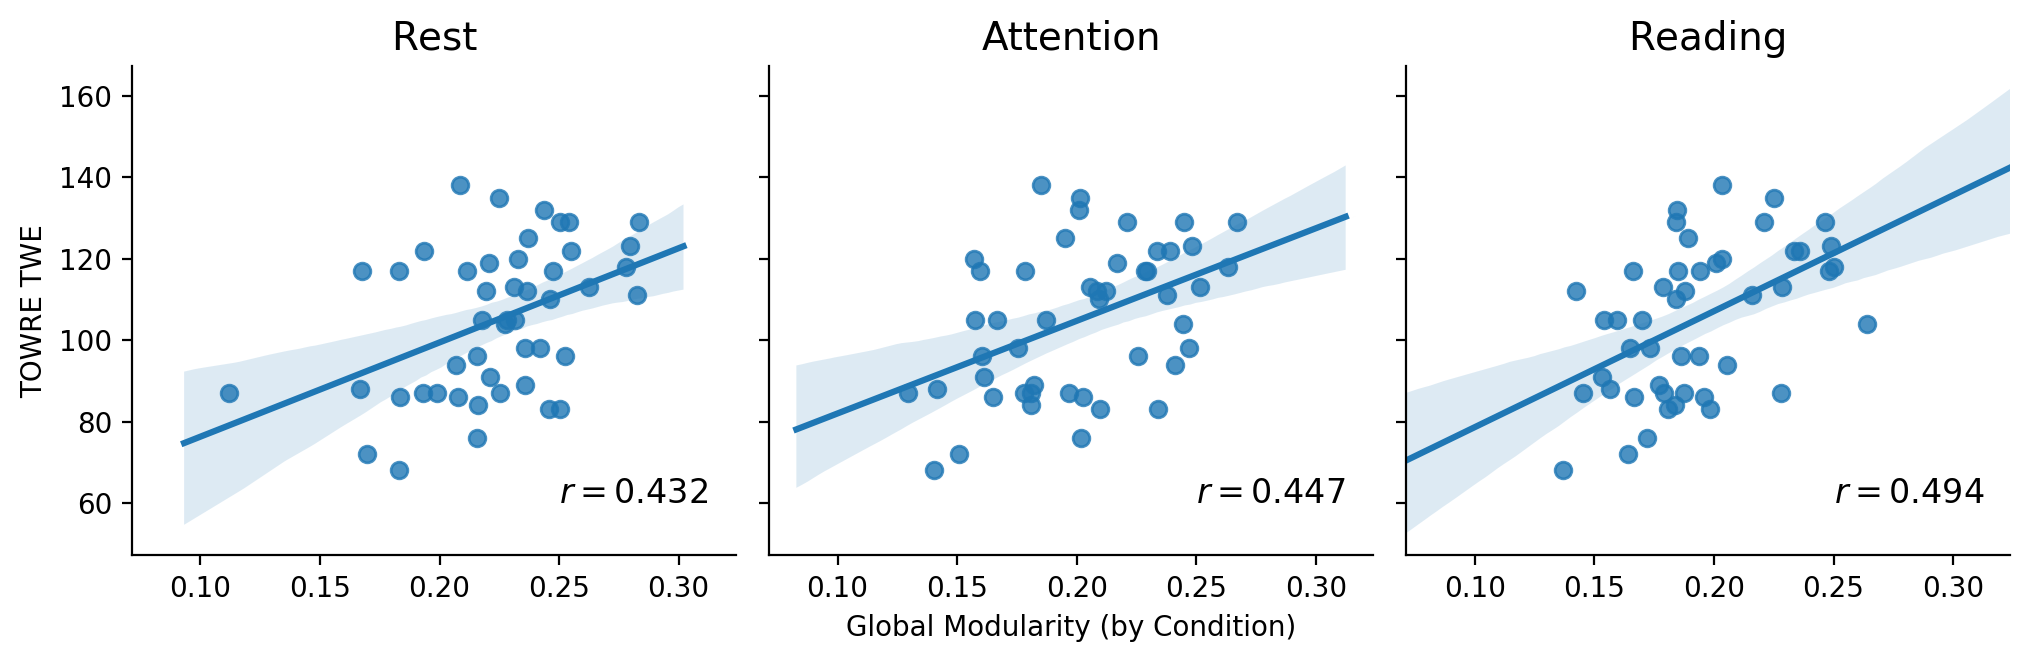
\includegraphics[width=6in]{ch3-modularity-reading-by-condition}
    \caption[Higher modularity in reading is also related to reading skill]{Higher modularity in reading is also related to reading skill. Although the global modularity significantly decreased for each subject, there was still a positive relationship between global modularity and reading skill.}
	\label{fig:ch3-modularity-reading-by-condition}
\end{figure}


\section{Discussion}

% Restatement of purpose and results
The primary purpose of the current study was to determine the ways in which task-evoked network architecture during reading differs from its baseline architecture, and whether changes in modularity are good predictors of better reading skill. As expected, we found that reading activated areas throughout the brain, especially in the visual, ventral attention and default mode networks. Reading also increased measures of integration throughout the brain compared to rest and a simple visual task. This integration was primarily driven by the de-clustering of sensory, dorsal attention and default RSNs, and global increases to the participation coefficients. Interestingly, we also found that hub areas -- those with the highest participation coefficients -- tended to be deactivated. Finally, we found that the positive direction of the relationship between modularity and reading skill was unchanged at rest and in task.

% Emphasize system-vs-laterality approach
One feature of the present connectomics approach is the disregard for laterality effects. There has traditionally been a major focus on laterality in reading and language \citep{Martin2015}. However, a systems-based approach aggregates across the RSN instead, providing a more comprehensive summary of the network's performance, but also making it less sensitive to task effects in processes that are strongly lateralized. However, there is much to be gained by prioritizing systems of the brain over sides. First, these right hemisphere regions are homologues of important left hemisphere language areas, and complement major processing areas such as the temporoparietal junction and angular gyrus \citep{Price2012, Jung-Beeman2005}. Secondly, the domain-general functions subserved by attention, executive and default networks are thought to be more global and less lateralized, so the broader scope is more appropriate when treating reading holistically (with less focus on decoding or semantics, for example) \citep{Yeo2011}.  

% Distribution of activity among different RSNs
One insight gained in this study is that much of the ``reading network'' falls predominantly in visual, default and ventral attention networks. The heavy engagement of ``unclassifiable'' border nodes is also indicative of the integrative nature of reading. While the visual and default mode networks are commonly discussed in reading comprehension as the seats of decoding and semantic processing, respectively, the attention networks have received less attention. The ventral attention network, which was the most comprehensively activated RSN in reading, plays a key role in integrating information from the environment, and regulating top-down attention. It has a push-pull relationship with the dorsal attention and salience networks. This can be seen in Figure \ref{fig:ch3-reading-connectome-activations}, where the VAN and DAN are activated in an oppposing manner. This relationship is important for reading: the dorsal attention network encompasses the visual word form area, which was the only activated DAN node and an area that has been the subject of much interest and debate in reading and dyslexia research \citep{McCandliss2003}. It is probable that this area is so important in reading not only because it is connected to language areas \citep{Bouhali2014}, but also because it is tightly tied to other areas that control goal-directed attention \citep{Vogel2014}. Vogel and colleagues found that reading ability in typical children and adults (including decoding and passage comprehension ability) predicted increased correlations between the visual word form area and the DAN \citep{Vogel2012a}. The nesting of this orthographic-processing area within the attention systems is further evidence of how fundamental global systems of attention are to the reading process.

% Changes to global modularity, but no changes to reading correlation
In terms of global network effects, we found that tasks reduced global measures of modularity and increased measures of between-RSN communication, including participation coefficient and path length. Relative to rest, this was most apparent in the visual RSN, which was characterized by a massive decrease in modularity compared to rest. These findings support a model in which the modular architecture of the brain is highly maintained between tasks, with global and some regional changes. It is not yet possible to say whether modularity within these specific RSNs correlates most highly with reading because of their functional roles in reading processes or whether they simply capture global trends better than other networks (because they are larger, for example). There is some reason to suspect specificity, however. In studies of remediation-induced changes to connectivity, increased connectivity within the visual network \citep{Koyama2013} and cingulo-opercular network \citep{HorowitzKraus2015} have predicted reading improvement in dyslexic children.

% Participation coefficient
Previous research have also noted that brain regions that have been found to be abnormal in dyslexia localize on high-hub regions \citep{Bailey2018}. It is perhaps surprising then to see primarily global effects of condition on the participation coefficient. However, this is consistent with the definition of the participation coefficient: the nodes that are increasing in participation coefficients are predominantly on the ``periphery'' of each RSN, and they are present in roughly equal proportions across all RSNs. Overall, however, we found that nodes with high participation coefficients tended not to be activated during reading, with a few exceptions such as the left posterior middle temporal gyrus. One explanation is that, in most cases, the nodes responsible for integrating information throughout the brain are not ``taxed'' in the same way that nodes performing specific computational processes are. The fronto-parietal network, for example, showed no RSN-level changes in activity, although it is known to play an important role in task-switching and coordinating neural systems \citep{Cole2013}. It is also possible that the frequency with which these hub areas are engaged varies, such that they do not activate in response to the stimuli but at other times. This anti-correlation between task activity and participation coefficient highlights the complementary nature of network analysis with activation analyses. 

% Overall significance 
Overall, the results suggest that the maintenance of an efficient network organization, i.e. one in which brain areas form clusters connected by hub regions, is important for skilled reading, even as between-network connectivity increases. To our knowledge, this is the first time the relationship between modularity and hubness to reading skill has been described during reading, adding to a foundation of work built on other connectivity methods. It also provides a replication of the resting-state findings described in Study 1. However, one limitation of the present approach is that effects were measured at a global level using the a pre-defined RSN parcellation. While this allows for reproducibility and an interpretable RSN ``rewiring'' framework, it cannot capture or describe the presence of new communities \citep{Power2011}. Comparing the modularity or individual connections between conditions assumes a reference framework, but to what extent is \textit{flexibility} in network connectivity important? Other analytical methods, such as investigating the number of shared connection between two connectomes may provide a more detailed insight into variability in task-evoked connectomes \citep{Petersen2015}. In the next chapter, we will address this question of how individual networks reorganize across a wider variety of tasks.
